%%%%%%%%%%%%%%%%%%%%%%%%%%%%%%%%%%%%%%%%%
% Masters/Doctoral Thesis 
% LaTeX Template
% Version 2.5 (27/8/17)
%
% This template was downloaded from:
% http://www.LaTeXTemplates.com
%
% Version 2.x major modifications by:
% Vel (vel@latextemplates.com)
%
% This template is based on a template by:
% Steve Gunn (http://users.ecs.soton.ac.uk/srg/softwaretools/document/templates/)
% Sunil Patel (http://www.sunilpatel.co.uk/thesis-template/)
%
% Template license:
% CC BY-NC-SA 3.0 (http://creativecommons.org/licenses/by-nc-sa/3.0/)
%
%%%%%%%%%%%%%%%%%%%%%%%%%%%%%%%%%%%%%%%%%

%----------------------------------------------------------------------------------------
%	PACKAGES AND OTHER DOCUMENT CONFIGURATIONS
%----------------------------------------------------------------------------------------

\documentclass[
% \openany
% \documentclass[openany]{book}
11pt, % The default document font size, options: 10pt, 11pt, 12pt
%oneside, % Two side (alternating margins) for binding by default, uncomment to switch to one side
english, % ngerman for German
singlespacing, % Single line spacing, alternatives: onehalfspacing or doublespacing
%draft, % Uncomment to enable draft mode (no pictures, no links, overfull hboxes indicated)
%nolistspacing, % If the document is onehalfspacing or doublespacing, uncomment this to set spacing in lists to single
%liststotoc, % Uncomment to add the list of figures/tables/etc to the table of contents
%toctotoc, % Uncomment to add the main table of contents to the table of contents
%parskip, % Uncomment to add space between paragraphs
%nohyperref, % Uncomment to not load the hyperref package
headsepline, % Uncomment to get a line under the header
%chapterinoneline, % Uncomment to place the chapter title next to the number on one line
%consistentlayout, % Uncomment to change the layout of the declaration, abstract and acknowledgements pages to match the default layout
]{MastersDoctoralThesis} % The class file specifying the document structure

\usepackage[utf8]{inputenc} % Required for inputting international characters
\usepackage[T1]{fontenc} % Output font encoding for international characters

\usepackage{mathpazo} % Use the Palatino font by default

\usepackage[backend=bibtex,style=authoryear,natbib=true]{biblatex} % Use the bibtex backend with the authoryear citation style (which resembles APA)

\addbibresource{example.bib} % The filename of the bibliography

\usepackage[autostyle=true]{csquotes} % Required to generate language-dependent quotes in the bibliography

%----------------------------------------------------------------------------------------
%	MARGIN SETTINGS
%----------------------------------------------------------------------------------------

\geometry{
	paper=a4paper, % Change to letterpaper for US letter
	inner=2.5cm, % Inner margin
	outer=3.8cm, % Outer margin
	bindingoffset=.5cm, % Binding offset
	top=1.5cm, % Top margin
	bottom=1.5cm, % Bottom margin
	%showframe, % Uncomment to show how the type block is set on the page
}



\thesistitle{Credit Card Fraud Detection} % Your thesis title, this is used in the title and abstract, print it elsewhere with \ttitle
\supervisor{Dr. Munnendra Ojha} % Your supervisor's name, this is used in the title page, print it elsewhere with \supname
\examiner{} % Your examiner's name, this is not currently used anywhere in the template, print it elsewhere with \examname
\degree{Information Technology} % Your degree name, this is used in the title page and abstract, print it elsewhere with \degreename
\author{Payal \textsc{Meena}} % Your name, this is used in the title page and abstract, print it elsewhere with \authorname
\addresses{} % Your address, this is not currently used anywhere in the template, print it elsewhere with \addressname

\subject{Biological Sciences} % Your subject area, this is not currently used anywhere in the template, print it elsewhere with \subjectname
\keywords{} % Keywords for your thesis, this is not currently used anywhere in the template, print it elsewhere with \keywordnames
\university{\href{http://www.university.com}{Indian Institute of Information technology Allahabad}} % Your university's name and URL, this is used in the title page and abstract, print it elsewhere with \univname
\department{\href{http://department.university.com}{Machine Learning}} % Your department's name and URL, this is used in the title page and abstract, print it elsewhere with \deptname
\group{\href{http://researchgroup.university.com}{5th Semester}} % Your research group's name and URL, this is used in the title page, print it elsewhere with \groupname
\faculty{\href{http://faculty.university.com}{Faculty Name}} % Your faculty's name and URL, this is used in the title page and abstract, print it elsewhere with \facname

\AtBeginDocument{
\hypersetup{pdftitle=\ttitle} % Set the PDF's title to your title
\hypersetup{pdfauthor=\authorname} % Set the PDF's author to your name
\hypersetup{pdfkeywords=\keywordnames} % Set the PDF's keywords to your keywords
}

\begin{document}

\frontmatter % Use roman page numbering style (i, ii, iii, iv...) for the pre-content pages

\pagestyle{plain} % Default to the plain heading style until the thesis style is called for the body content

%----------------------------------------------------------------------------------------
%	TITLE PAGE
%----------------------------------------------------------------------------------------

\begin{titlepage}
\begin{center}

% \vspace*{.06\textheight}
{\scshape\LARGE \univname\par}\vspace{1.5cm} % University name
\textsc{\Large Course Project}\\[0.5cm] % Thesis type

\HRule \\[0.4cm] % Horizontal line
{\huge \bfseries \ttitle\par}\vspace{0.4cm} % Thesis title
\HRule \\[1.5cm] % Horizontal line
 
\begin{minipage}[t]{0.4\textwidth}
\begin{flushleft} \large
\emph{Author:}\\
\href{http://www.johnsmith.com}{\authorname} % Author name - remove the \href bracket to remove the link
\end{flushleft}
\end{minipage}
\begin{minipage}[t]{0.4\textwidth}
\begin{flushright} \large
\emph{Supervisor:} \\
\href{http://www.jamessmith.com}{\supname} % Supervisor name - remove the \href bracket to remove the link  
\end{flushright}
\end{minipage}\\[3cm]
 
% \vfill

\large \textit{A course project is submitted in fulfillment of the requirements\\ for the degree of \degreename}\\[0.3cm] % University requirement text
\textit{in the}\\[0.4cm]
\groupname\\\deptname\\[2cm] % Research group name and department name
 
% \vfill

{\large \today}\\[4cm] % Date
%\includegraphics{Logo} % University/department logo - uncomment to place it
% \vfill
\end{center}
\end{titlepage}
\let\cleardoublepage\clearpage

% \begin{declaration}
% \addchaptertocentry{\authorshipname}
% \noindent I, \authorname, declare that this thesis titled, \enquote{\ttitle} and the work presented in it are my own. I confirm that:

% \begin{itemize} 
% \item This work was done wholly or mainly while in candidature for a B.Tech degree at this University.
% \item Where any part of this thesis has previously been submitted for a degree or any other qualification at this University or any other institution, this has been clearly stated.
% \item Where I have consulted the published work of others, this is always clearly attributed.
% \item Where I have quoted from the work of others, the source is always given. With the exception of such quotations, this thesis is entirely my own work.
% \item I have acknowledged all main sources of help.
% \item Where the thesis is based on work done by myself jointly with others, I have made clear exactly what was done by others and what I have contributed myself.
% \end{itemize}
 
% \noindent Signed:
% \rule[0.5em]{25em}{0.5pt} 
 
% \noindent Date:
% \rule[0.5em]{25em}{0.5pt}
% \end{declaration}

% \cleardoublepage
% \clearpage


% \vspace*{0.2\textheight}

\tableofcontents % Prints the main table of contents
\let\cleardoublepage\clearpage
%----------------------------------------------------------------------------------------
%	ABSTRACT PAGE
%----------------------------------------------------------------------------------------

\begin{abstract}
\addchaptertocentry{\abstractname} % Add the abstract to the table of contents
The project is mainly focussed on credit card
fraud detection in real world. A phenomenal growth in the
number of credit card transactions, has recently led to a
considerable rise in fraudulent activities. The purpose is to
obtain goods without paying, or to obtain unauthorized funds
from an account. Implementation of efficient fraud detection
systems has become imperative for all credit card issuing
banks to minimize their losses. One of the most crucial
challenges in making the business is that neither the card nor
the cardholder needsto be present when the purchase is being
made. This makes it impossible for the merchant to verify
whether the customer making a purchase is the authentic
cardholder or not. With the proposed scheme, using random
forest algorithm the accuracy of detecting the fraud can be
improved can be improved. Classification process of random
forest algorithm to analyse data set and user current dataset.
Finally optimize the accuracy of the result data. The
performance of the techniques is evaluated based on accuracy,
sensitivity, and specificity, and precision. Then processing of
some of the attributes provided identifies the fraud detection
and provides the graphical model visualization. The
performance of the techniques is evaluated based on accuracy,
sensitivity, and specificity, and precision.
\ldots
\end{abstract}
\let\cleardoublepage\clearpage

\begin{acknowledgements}
\addchaptertocentry{\acknowledgementname} % Add the acknowledgements to the table of contents
I extend my sincere gratitude to everyone who played a role in the successful completion of this individual project on credit card fraud detection.

First and foremost, I express my deepest appreciation to Dr. Munnendra Ojha, whose guidance and expertise provided invaluable direction throughout the entire project. Their insights and encouragement fueled my motivation and enhanced the quality of the work.

A special thank you to IIITA for granting access to the necessary datasets and resources, enabling me to delve into the intricacies of credit card transactions and fraud patterns.

I would also like to acknowledge the support of our TA Arindnam Ghosh for their constructive feedback and discussions that greatly contributed to refining the methodology and approach of the fraud detection system.

This project has been a solitary endeavor, but not without the encouragement of friends and family. I am grateful for their understanding, patience, and encouragement during the intensive phases of research and analysis.

In conclusion, I appreciate the opportunity to work on a project of such significance, and I am thankful for the guidance, support, and resources provided by all those involved.\ldots
\end{acknowledgements}
\let\cleardoublepage\clearpage
%----------------------------------------------------------------------------------------
%	LIST OF CONTENTS/FIGURES/TABLES PAGES
%----------------------------------------------------------------------------------------

% \tableofcontents % Prints the main table of contents
% \let\cleardoublepage\clearpage
% \listoffigures % Prints the list of figures

% \listoftables % Prints the list of tables

%----------------------------------------------------------------------------------------
%	ABBREVIATIONS
%----------------------------------------------------------------------------------------

% \begin{abbreviations}{ll} % Include a list of abbreviations (a table of two columns)

% \textbf{LAH} & \textbf{L}ist \textbf{A}bbreviations \textbf{H}ere\\
% \textbf{WSF} & \textbf{W}hat (it) \textbf{S}tands \textbf{F}or\\

% \end{abbreviations}

%----------------------------------------------------------------------------------------
%	PHYSICAL CONSTANTS/OTHER DEFINITIONS
%----------------------------------------------------------------------------------------

% \begin{constants}{lr@{${}={}$}l} % The list of physical constants is a three column table

% % The \SI{}{} command is provided by the siunitx package, see its documentation for instructions on how to use it

% Speed of Light & $c_{0}$ & \SI{2.99792458e8}{\meter\per\second} (exact)\\
% %Constant Name & $Symbol$ & $Constant Value$ with units\\

% \end{constants}

%----------------------------------------------------------------------------------------
%	SYMBOLS
%----------------------------------------------------------------------------------------

% \begin{symbols}{lll} % Include a list of Symbols (a three column table)

% $a$ & distance & \si{\meter} \\
% $P$ & power & \si{\watt} (\si{\joule\per\second}) \\
% %Symbol & Name & Unit \\

% \addlinespace % Gap to separate the Roman symbols from the Greek

% $\omega$ & angular frequency & \si{\radian} \\

% \end{symbols}

%----------------------------------------------------------------------------------------
%	DEDICATION
%----------------------------------------------------------------------------------------

% \dedicatory{For/Dedicated to/To my\ldots} 

%----------------------------------------------------------------------------------------
%	THESIS CONTENT - CHAPTERS
%----------------------------------------------------------------------------------------

\mainmatter % Begin numeric (1,2,3...) page numbering

\pagestyle{thesis} % Return the page headers back to the "thesis" style

% Include the chapters of the thesis as separate files from the Chapters folder
% Uncomment the lines as you write the chapters

% Chapter 1
\let\cleardoublepage\clearpage
 % \let\cleardoublepage\clearpage
\chapter{Introduction} % Main chapter title

\label{Chapter1} % For referencing the chapter elsewhere, use \ref{Chapter1} 

%----------------------------------------------------------------------------------------

% Define some commands to keep the formatting separated from the content 
\newcommand{\keyword}[1]{\textbf{#1}}
\newcommand{\tabhead}[1]{\textbf{#1}}
\newcommand{\code}[1]{\texttt{#1}}
\newcommand{\file}[1]{\texttt{\bfseries#1}}
\newcommand{\option}[1]{\texttt{\itshape#1}}

%----------------------------------------------------------------------------------------
\section{Background}
Credit card fraud is a persistent challenge in the financial landscape, with criminals constantly devising new methods to exploit vulnerabilities. This project aims to develop an effective credit card fraud detection system using advanced machine learning techniques.\medskip

The credit card has become the most popular payment method for both online and offline transactions. The necessity to create a fraud detection algorithm to precisely identify and stop fraudulent activity arises as a result of both the development of technology and the rise in fraud cases

\section{About}
There are various fraudulent activities detection techniques
has implemented in credit card transactions have been kept
in researcher minds to methods to develop models based on
artificial intelligence , data mining, fuzzy logic and machine
learning. Credit card fraud detection is significantly difficult,
but also popular problem to solve. In our proposed system
we built the credit card fraud detection using Machine
learning. With the advancement of machine learning
techniques. Machine learning has been identified as a
successful measure for fraud detection. A large amount of
data is transferred during online transaction processes,
resulting in a binary result: genuine or fraudulent. Within the
sample fraudulent datasets, features are constructed. These
are data points namely the age and value of the customer
account, as well as the origin of the credit card. There are
hundreds of features and each contributes, to varying
extents, towards the fraud probability. Note, the level in
which each feature contributes to the fraud score is
generated by the artificial intelligence of the machine which
is driven by the training set, but is not determined by a fraud analyst. \medskip

So, in regards to the card fraud, if the use of cards to
commit fraud is proven to be high, the fraud weighting of a
transaction that uses a credit card will be equally so.
However, if this were to shrink, the contribution level would
parallel. Simply make, these models self-learn without
explicit programming such as with manual review. Credit
card fraud detection using Machine learning is done by
deploying the classification and regression algorithms. We
use supervised learning algorithm such as Random forest
algorithm to classify the fraud card transaction in online or
by offline. Random forest is advanced version of Decision
tree. Random forest has better efficiency and accuracy than
the other machine learning algorithms. Random forest aims
to reduce the previously mentioned correlation issue by
picking only a subsample of the feature space at each
split. Essentially, it aims to make the trees de-correlated
and prune the trees by fixing a stopping criteria for node
splits, which I will be cover in more detail later.

%----------------------------------------------------------------------------------------
% \let\cleardoublepage\clearpage
\section{Problem Definition}

Billions of dollars of loss are caused every year by the
fraudulent credit card transactions. Fraud is old as humanity
itself and can take an unlimited variety of different forms.
The PwC global economic crime survey of 2017 suggests that
approximately 48% of organizations experienced economic
crime. Therefore, there is definitely an urge to solve the
problem of credit card fraud detection.Moreover, the
development of new technologies provides additional ways
in which criminals may commit fraud. The use of credit cards
is prevalent in modern day society and credit card fraud has
been kept on growing in recent years. Hugh Financial losses
has been fraudulent affects not only merchants and banks,
but also individual person who are using the credits. Fraud
may also affect the reputation and image of a merchant
causing non-financial losses that, though difficult to quantify
in the short term, may become visible in the long period. For
example, if a cardholder is victim of fraud with a certain
company, he may no longer trust their business and choose a
contender.

\section{Scope of the Project}

In this proposed project we designed a protocol or a model
to detect the fraud activity in credit card transactions.
This system is capable of providing most of the essential
features required to detect fraudulent and legitimate
transactions. As technology changes, it becomes difficult to track the
behaviour and pattern of fraudulent transactions.
With the upsurge of machine learning, artificial intelligence
and other relevant fields of information technology, it
becomes feasible to automate the process and to save some
of the effective amount of labor that is put into detecting
credit card fraudulent activities.\medskip

The scope of this project revolves around leveraging advanced machine learning techniques, specifically Random Forest and Logistic Regression, to fortify credit card fraud detection systems. The aim is to enhance the accuracy, efficiency, and adaptability of the current fraud detection methodology, addressing the challenges posed by imbalanced datasets and the ever-evolving nature of fraudulent activities.


















%----------------------------------------------------------------------------------------


%----------------------------------------------------------------------------------------






%----------------------------------------------------------------------------------------







% Chapter 2
\let\cleardoublepage\clearpage
 % \let\cleardoublepage\clearpage
\chapter{Literature Review} % Main chapter title

\label{Chapter2} % For referencing the chapter elsewhere, use \ref{Chapter1} 

%----------------------------------------------------------------------------------------

% Define some commands to keep the formatting separated from the content 
\newcommand{\keyword}[1]{\textbf{#1}}
\newcommand{\tabhead}[1]{\textbf{#1}}
\newcommand{\code}[1]{\texttt{#1}}
\newcommand{\file}[1]{\texttt{\bfseries#1}}
\newcommand{\option}[1]{\texttt{\itshape#1}}

\section{Overview of Credit Card Fraud Detection}

Credit card fraud represents a persistent and evolving threat in the financial ecosystem, where malicious actors seek to exploit vulnerabilities in payment systems for personal gain. This section provides an insightful overview of credit card fraud, shedding light on the tactics employed by fraudsters and the dynamic landscape of fraudulent activities.



Credit card fraud manifests in various forms, including:\medskip 
\begin{itemize}
    \item According to the Nilson Report, global card fraud losses were estimated to be around \$27.85 billion in 2018.\medskip 

    \item  The Federal Trade Commission (FTC) reported that credit card fraud represented a significant portion of identity theft cases, with around 33\% of all reported cases in 2020.\medskip 

    \item According to Visa, merchants who have completed the EMV chip upgrade saw a 76\% drop in counterfeit fraud from December 2015 to March 2018.\medskip 

    
    
    \item  The LexisNexis True Cost of Fraud Study 2019 reported that for every dollar of fraud, merchants incurred an additional \$3.13 billion in costs.\medskip

    \item  Depending on the complexity and the dataset used, have reported accuracies ranging from 85\% to 99\%.\medskip

    \item  Balancing the detection of fraudulent activity with minimizing false positives is a constant challenge. False positive rates for some models have been reported in the range of 1\% to 5\%.\medskip
\end{itemize}

\subsection{Evolution of Credit Card Fraud:}

As technology advances, so do the methods employed by fraudsters. The emergence of online transactions and digital payment methods has introduced new vectors for exploitation, necessitating innovative and adaptive fraud detection measures.\medskip

Understanding the multifaceted nature of credit card fraud is crucial for developing effective detection systems that can anticipate and thwart the ever-changing strategies of malicious actors. In the subsequent sections, we delve into the existing methods and the application of machine learning, particularly the Random Forest Classifier, to fortify credit card fraud detection mechanisms.






%----------------------------------------------------------------------------------------

\section{Existing Fraud Detection Methods}

\subsection{Random Forest}

Random forest is a type of supervised machine learning
algorithm based on ensemble learning. Ensemble learning is
a type of learning where you join different types of
algorithms or same algorithm multiple times to form a more
powerful prediction model. The random forest algorithm
combines multiple algorithm of the same type i.e. multiple
decision trees, resulting in a forest of trees, hence the name
"Random Forest". The random forest algorithm can be used
for both regression and classification tasks.\medskip

\keyword{WORKING OF RANDOM FOREST } 
\begin{itemize}
\item 1. Pick N random records from the dataset.
\item 2. Build a decision tree based on these N records.
\item 3. Choose the number of trees you want in your
algorithm and repeat steps 1 and 2.
\item 4. For classification problem, each tree in the forest
predicts the category to which the new record belongs.
Finally, the new record is assigned to the category that
wins the majority vote..\medskip
\end{itemize}
\keyword{Advantages of using Random Forest}
\begin{itemize}
\item  The random forest algorithm is not biased, since,
there are multiple trees and each tree is trained on a
subset of data. Basically, the random forest algorithm
relies on the power of "the crowd"; therefore, the
overall biasedness of the algorithm is reduced.
\item  This algorithm is very stable. Even if a new data
point is introduced in the dataset the overall algorithm
is not affected much since new data may impact one
tree, but it is very hard for it to impact all the trees.
\item  The random forest algorithm works well when you
have both categorical and numerical features.

\subsection{Logistic Regression}
Logistic regression is another powerful supervised ML algorithm used for binary classification problems (when target is categorical). The best way to think about logistic regression is that it is a linear regression but for classification problems. The primary difference between linear regression and logistic regression is that logistic regression's range is bounded between 0 and 1. In addition, as opposed to linear regression, logistic regression does not require a linear relationship between inputs and output variables.Logistic regression is based on the sigmoid function and its result is from zero to one. 
\medskip
\begin{figure}[h]
    \centering
    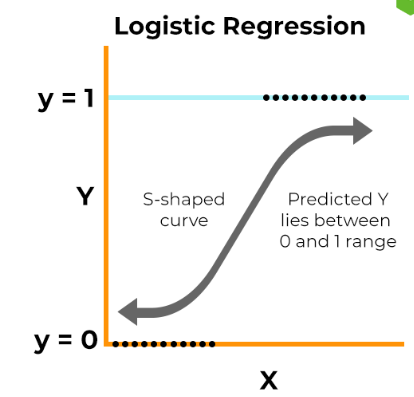
\includegraphics[width=0.5\linewidth]{image1.png}
    \caption{Logistic Regression}
    \label{fig:enter-label}
\end{figure}
\keyword{Advantages of using Logistic Regression}
\item Logistic regression provides easily interpretable results. The coefficients assigned to each feature indicate the strength and direction of their influence on the likelihood of fraud. This transparency is crucial for understanding the factors contributing to fraud.

\item It's computationally efficient, especially when compared to more complex models. This efficiency becomes important when dealing with large datasets, a common scenario in credit card transactions.

\item Credit card fraud detection is essentially a binary classification problem (fraud or not fraud). Logistic regression is specifically designed for such scenarios and is well-suited for predicting probabilities associated with two outcomes.
\item If the data can be separated by a straight line (or hyperplane in higher dimensions), logistic regression performs well. In many cases, fraud detection features may exhibit a linear relationship with the likelihood of fraud, making logistic regression a suitable choice.





\end{itemize}
 
% Chapter 3
\let\cleardoublepage\clearpage
 % \let\cleardoublepage\clearpage
\chapter{Methdology} % Main chapter title

\label{Chapter3} % For referencing the chapter elsewhere, use \ref{Chapter1} 

%----------------------------------------------------------------------------------------

% Define some commands to keep the formatting separated from the content 
\newcommand{\keyword}[1]{\textbf{#1}}
\newcommand{\tabhead}[1]{\textbf{#1}}
\newcommand{\code}[1]{\texttt{#1}}
\newcommand{\file}[1]{\texttt{\bfseries#1}}
\newcommand{\option}[1]{\texttt{\itshape#1}}


\section{Data Collection}

In the pursuit of building an effective credit card fraud detection system, a critical initial step involves the collection and understanding of the data that will fuel the model's learning. This section outlines the process of importing necessary libraries, loading the dataset, and gaining insights into its structure.\medskip

In the context of machine learning, the effectiveness of our model is highly dependent on the quality of the dataset we use. Prior to delving into the nuances of model development, a pivotal phase involves the preprocessing of your dataset. This encompasses addressing missing values, handling duplicates, and transforming variables into a format that is conducive for model comprehension. This chapter delves into the intricate steps of data preprocessing undertaken for a credit card fraud detection project.

\subsection{Data Sources}

The project will utilize real credit card transaction data obtained from the kaggle which contains transactions made by credit cards in September 2013 by European cardholders.This dataset presents transactions that occurred in two days, where we have 492 frauds out of 284,807 transactions. The dataset is highly unbalanced, the positive class (frauds) account for 0.172\% of all transactions.\medskip

It contains only numerical input variables which are the result of a PCA transformation. Unfortunately, due to confidentiality issues, we cannot provide the original features and more background information about the data. Features V1, V2, … V28 are the principal components obtained with PCA, the only features which have not been transformed with PCA are 'Time' and 'Amount'. Feature 'Time' contains the seconds elapsed between each transaction and the first transaction in the dataset. The feature 'Amount' is the transaction Amount, this feature can be used for example-dependant cost-sensitive learning. Feature 'Class' is the response variable and it takes value 1 in case of fraud and 0 otherwise.

\subsection{Data Preprocessing}
\begin{itemize}
    \item \textbf{Data Cleaning:-} Before diving into the heart of the analysis, it's essential to ensure that the dataset is free from inconsistencies, missing values, and anomalies that could hinder the performance of our fraud detection system.

    \item \textbf{Feature Selection:-} Identifying the most relevant features (variables) is key to building an efficient model. This involves understanding the significance of each attribute and its potential contribution to the detection of fraudulent transactions.

    \item \textbf{Handling Imbalanced Data:-} Credit card fraud datasets often suffer from class imbalance, where the number of non-fraudulent transactions far exceeds fraudulent ones. Balancing the dataset is crucial to avoid the model being biased towards the majority class.

    \item \textbf{ Data Normalization:-}  Ensuring uniform scales across features is essential for certain machine learning algorithms. In the case of credit card fraud detection, normalizing the data aids in better convergence during the model training process.
    
\begin{figure}[h]
    \centering
    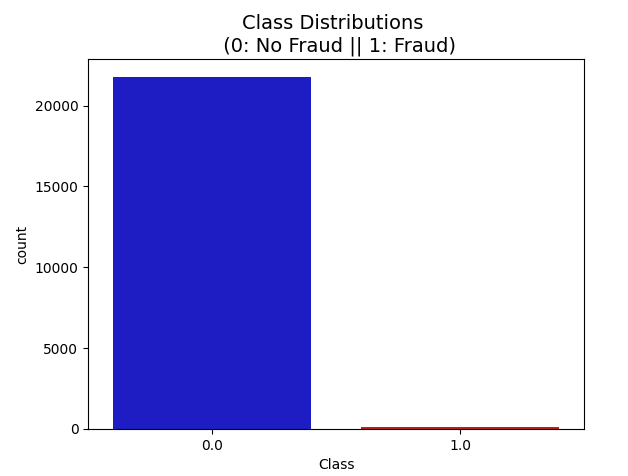
\includegraphics[width=0.7\linewidth]{image2.png}
    \caption{Class Distribution}
    \label{fig:enter-label}
\end{figure}

\item \textbf{ Scaling and Distributing :-}In this phase of our kernel, we will first scale the columns comprise of Time and Amount . Time and amount should be scaled as the other columns. On the other hand, we need to also create a sub sample of the dataframe in order to have an equal amount of Fraud and Non-Fraud cases, helping our algorithms better understand patterns that determines whether a transaction is a fraud or not.

 \begin{figure}[h]
    \centering
    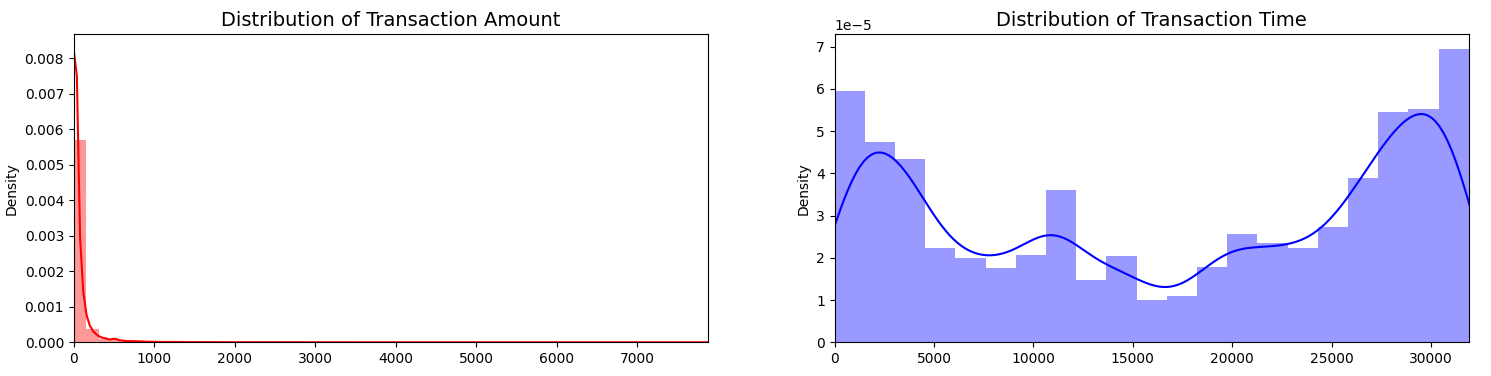
\includegraphics[width=0.8\linewidth]{image3.png}
    \caption{Distribution}
    \label{fig:enter-label}
 \end{figure}

\item \textbf{ Splitting Data:-}Before proceeding with the Random UnderSampling technique we have to separate the orginal dataframe. Why? for testing purposes, remember although we are splitting the data when implementing Random UnderSampling or OverSampling techniques, we want to test our models on the original testing set not on the testing set created by either of these techniques. The main goal is to fit the model either with the dataframes that were undersample and oversample (in order for our models to detect the patterns), and test it on the original testing set.

\end{itemize}

\section{Feature Selection/Engineering}

The process of identifying the most influential features and potentially creating new ones is critical for developing a robust credit card fraud detection model. This section delves into the methods employed for feature selection and engineering to enhance the overall efficacy of the model.\medskip

In my code, explicit feature selection techniques are not applied. Instead, the focus is on outlier detection and removal, correlation analysis, and subsampling to address class imbalance. Let's discuss how feature-related aspects are handled in the code.

\begin{itemize}
    \item \textbf{Feature Importance:-} Determining the importance of each feature provides insights into which variables significantly contribute to the identification of fraudulent transactions. Random Forest Classifier, being an ensemble method, inherently provides a mechanism to gauge feature importance.
    
    \item Correlation matrices (corr and sub\_sample\_corr) are used to visualize the correlation between features and the target variable ('Class').
    \item Features with high positive or negative correlations with the target variable are identified.
    \begin{figure}[h]
        \centering
        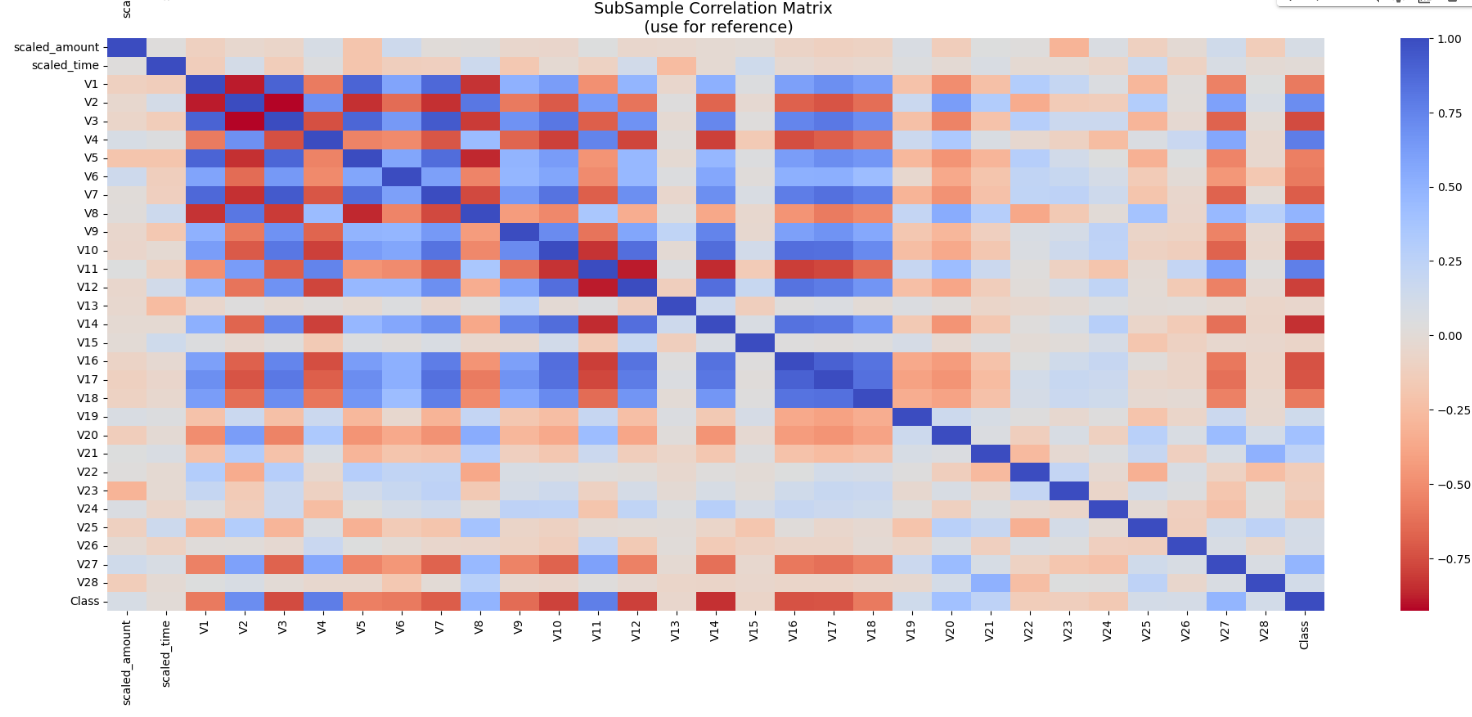
\includegraphics[width=0.9\linewidth]{image4.png}
        \caption{SubSample Correlation Matrix}
        \label{fig:enter-label}
    \end{figure}
    \item Boxplots are created to show the distribution of features with the highest negative and positive correlations.

  \item \textbf{Feature Engineering:-} Creating new features based on existing ones can uncover hidden patterns and improve the model's ability to discern fraudulent transactions.

  Feature selection and engineering are iterative processes, and the chosen techniques depend on the dataset and the behavior of fraudulent transactions. The selected features and engineered variables form the foundation for training and optimizing the Random Forest Classifier and Logistic Regression in the subsequent stages of the project.
   \begin{figure}[h]
       \centering
       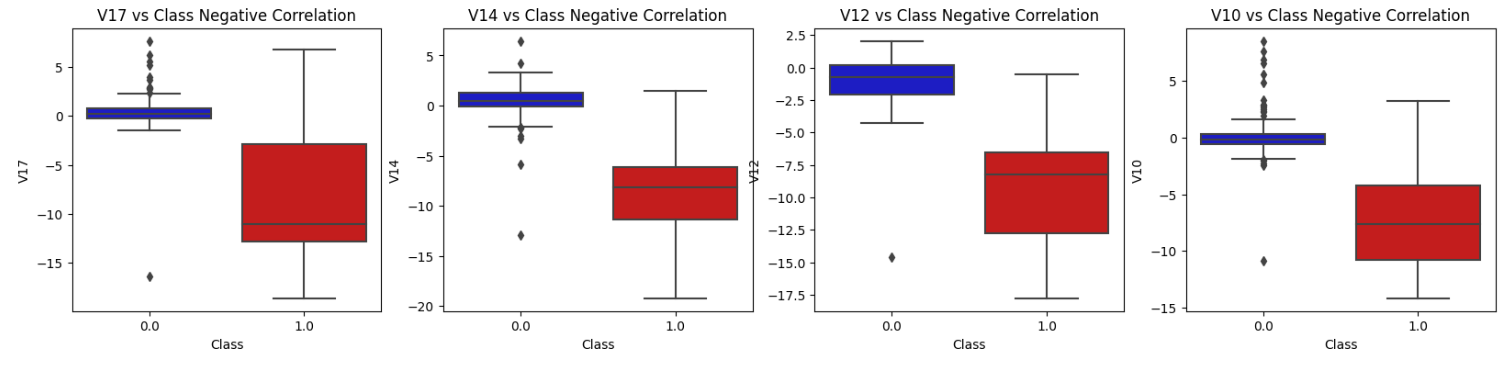
\includegraphics[width=0.9\linewidth]{image5.png}
       \caption{Negative Correlation With Classes}
       \label{fig:enter-label}
   \end{figure}
   \item \textbf{Outlier Detection:} Outlier detection in credit card fraud detection involves identifying and handling transactions that deviate significantly from the typical behavior of legitimate transactions. Outliers in this context are often indicative of potential fraudulent activity. 
   \item Outlier removal is performed for features V14, V12, and V10 using the interquartile range (IQR) method.
   
   \begin{figure}[h]
    \centering
    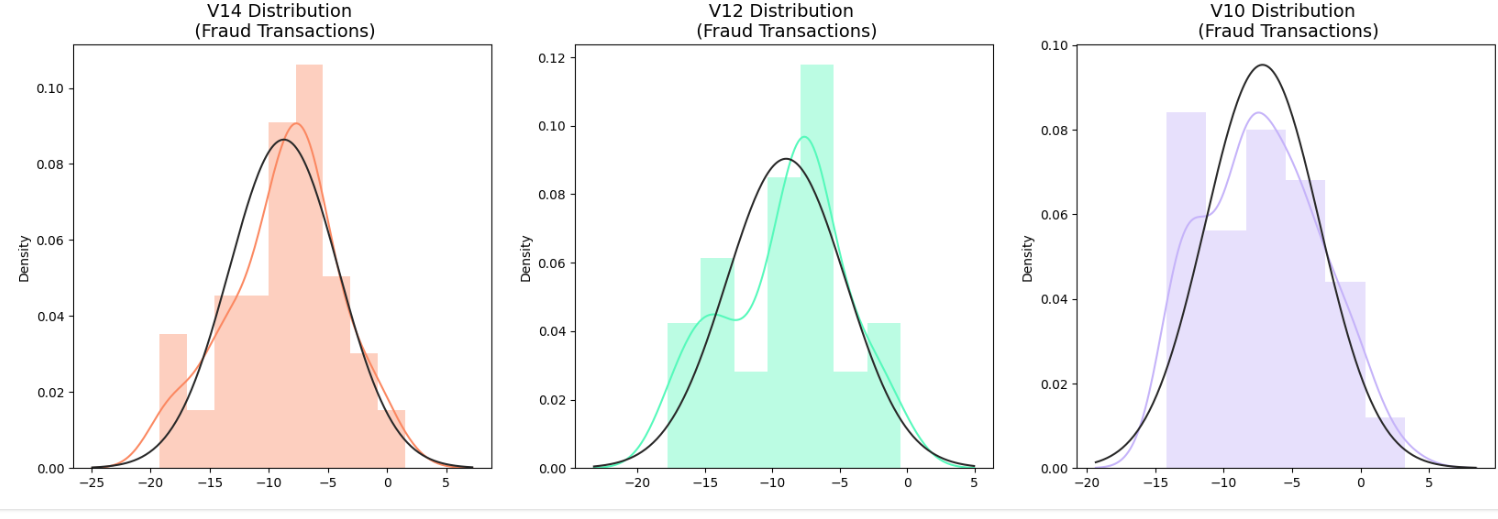
\includegraphics[width=0.9\linewidth]{image6.png}
    \caption{Fraud Transaction}
    \label{fig:enter-label}
\end{figure}

   \item The reduction in extreme outliers is visualized using boxplots.
   
   \begin{figure}[h]
       \centering
       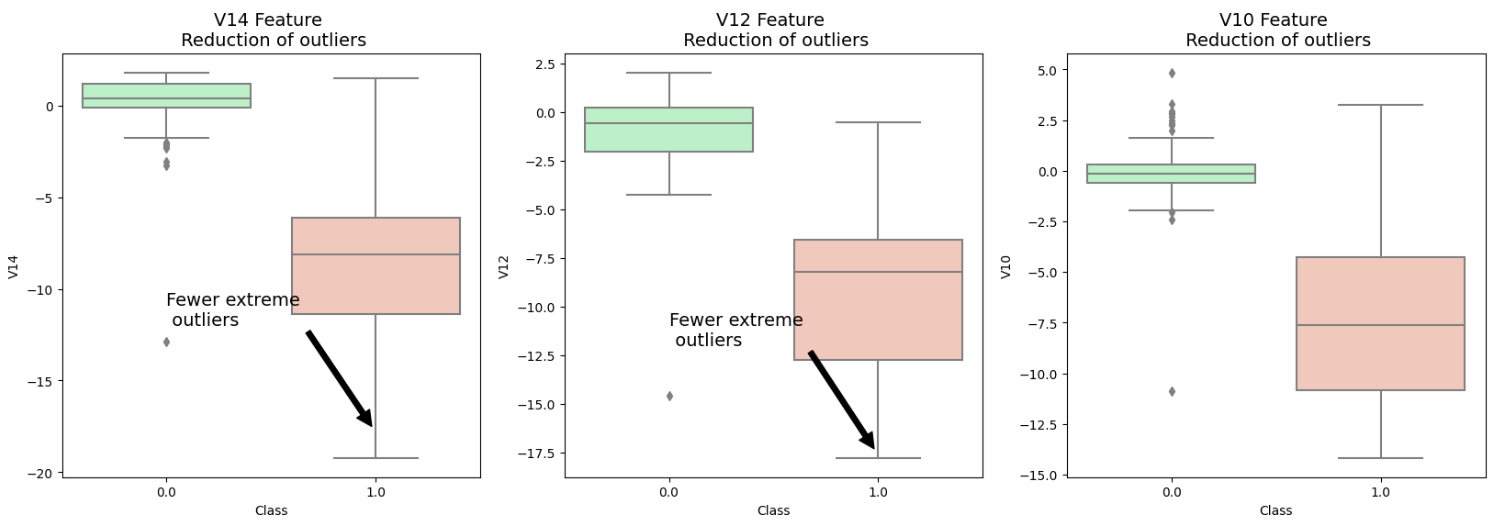
\includegraphics[width=0.9\linewidth]{image7.png}
       \caption{Reduction of Outliers}
       \label{fig:enter-label}
   \end{figure}

   \item \textbf{Subsampling:} Subsampling in the context of credit card fraud detection involves creating a balanced dataset by randomly selecting a subset of legitimate transactions to match the number of fraudulent transactions. This technique is often employed when dealing with imbalanced datasets, where fraudulent transactions are significantly less frequent than legitimate ones. 
   \item Random under-sampling is applied to balance the class distribution, ensuring an equal number of fraud and non-fraud instances.
   \item This subsample is then used for further analysis and model training.\medskip
   
  \item \textbf{Dimensionality Reduction and Clustering:} 
The dimensionality reduction techniques of t-SNE, PCA, and Truncated SVD were employed to visualize clusters in the credit card fraud dataset. The scatter plots showcase distinct clusters that differentiate between legitimate transactions (labeled as 'No Fraud') and fraudulent transactions (labeled as 'Fraud'). In the t-SNE plot, clusters exhibit a well-defined separation, highlighting the ability of t-SNE to capture complex patterns in high-dimensional data. PCA also effectively distinguishes between the two classes, revealing clusters with clear boundaries. Truncated SVD, while offering dimensionality reduction, demonstrates slightly overlapping clusters, indicating some level of complexity in the underlying data structure. The use of different dimensionality reduction techniques provides valuable insights into the distribution of fraud and non-fraud instances, aiding in the identification of patterns crucial for fraud detection in the credit card transactions dataset.

\begin{figure}[h]
    \centering
    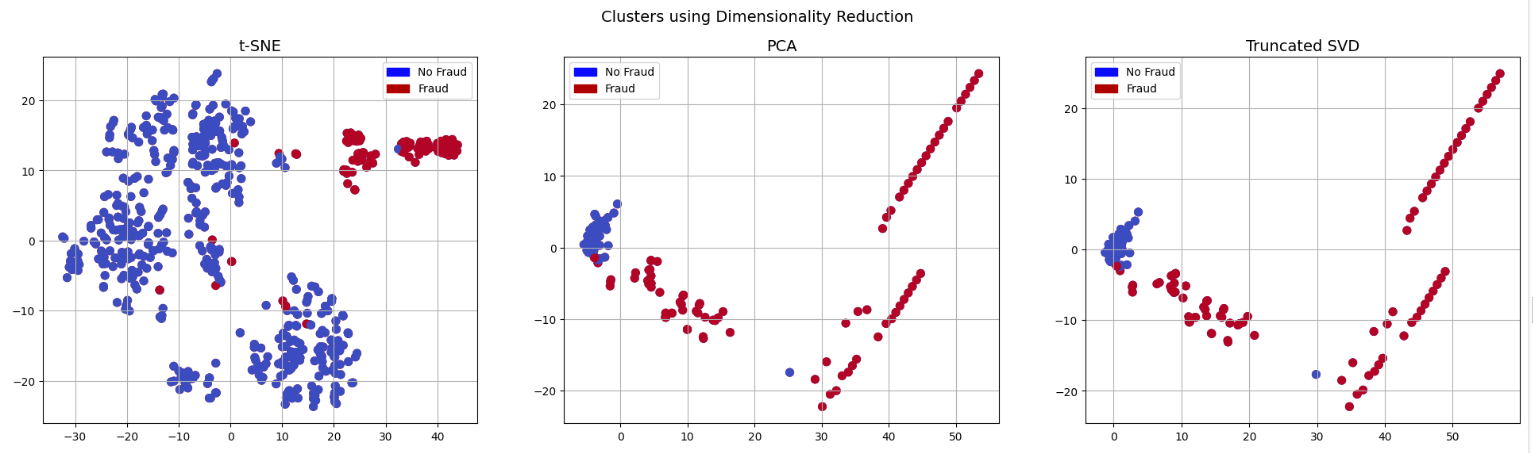
\includegraphics[width=0.9\linewidth]{image8.png}
    \caption{Clusters using Diamensionality}
    \label{fig:enter-label}
\end{figure}

   

\end{itemize}

\section{Model Selection:-} In credit card fraud detection, the choice of an appropriate model plays a pivotal role in achieving accurate and efficient results. The Random Forest Classifier and Logistic Regression stands out as a formidable choice due to its ability to handle complex patterns, manage large datasets, and mitigate overfitting, all crucial aspects in the context of identifying fraudulent transactions. Comprising an ensemble of decision trees, the Random Forest algorithm excels in capturing intricate relationships within the data, making it well-suited for the dynamic and evolving nature of credit card fraud. Leveraging the strength of multiple trees, it excels in delivering robust predictions and is inherently resistant to outliers and noise. The adaptability and resilience of the Random Forest Classifier position it as a reliable tool for our credit card fraud detection endeavor, promising to provide a nuanced understanding of transaction patterns and effectively differentiate between legitimate and fraudulent activities.\medskip

Logistic regression stands as a powerful ally in the ongoing battle against credit card fraud. Its simplicity, interpretability, and efficiency make it a valuable tool for financial institutions striving to protect their customers and maintain the integrity of electronic transactions. As technology evolves, logistic regression remains a steadfast and reliable solution in the realm of fraud detection.

\section{Evaluation:-} After the training phase, assessing the performance of the credit card fraud detection model is crucial to ensuring its efficacy in real-world scenarios. This section discusses the evaluation process and the metrics employed to gauge the model's success in accurately identifying fraudulent transactions.

\begin{itemize}

    \item \textbf{Accuracy:-} Accuracy represents the proportion of correctly classified instances, measuring the overall correctness of the model's predictions.This suggests that, during cross-validation on the training data, the Logistic Regression model achieved an accuracy of 85.0\% where the Random Forest give accuracy is 79\%. This high accuracy score indicates that, based on the training data, the Logistic Regression model is performing well in predicting whether transactions are fraudulent or not.

 \begin{figure}[h]
     \centering
     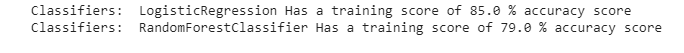
\includegraphics[width=0.9\linewidth]{image9.png}
     \caption{Accuracy Score}
     \label{fig:enter-label}
 \end{figure}
 
    \item \textbf{Precision and Recall:-} Precision and recall are particularly relevant in fraud detection. Precision measures the accuracy of positive predictions, while recall gauges the model's ability to capture all positive instances.\medskip
    
    \begin{figure}[h]
        \centering
        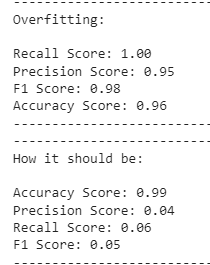
\includegraphics[width=0.5\linewidth]{image11.png}
        \caption{Precision and Recall score of LR}
        \label{fig:enter-label}
    \end{figure}
    
    This suggests that the ROC AUC score for the Logistic Regression model on the training data is 0.96 where the Random Forest gave 0.95, indicating a strong ability of the model to distinguish between positive and negative classes (fraudulent and legitimate transactions). Higher ROC AUC values generally imply better model performance.
    
    \begin{figure}[h]
        \centering
        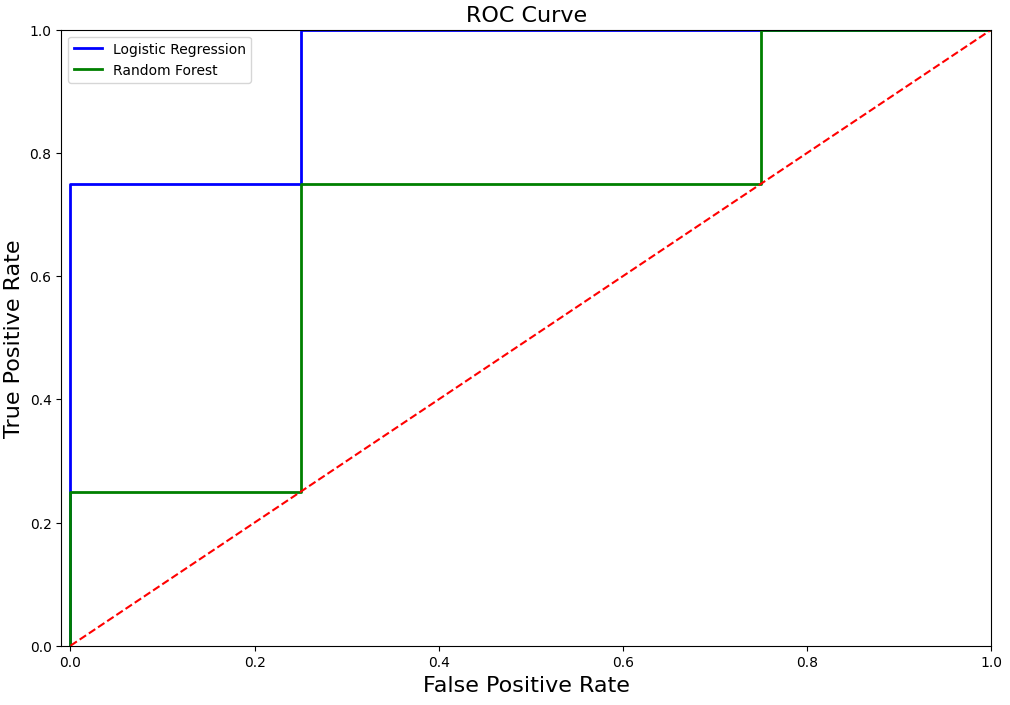
\includegraphics[width=0.9\linewidth]{image10.png}
        \caption{ROC Curve of LR and RF}
        \label{fig:enter-label}
    \end{figure}

    \item \textbf{Confusion Matrix:-} A confusion matrix provides a detailed breakdown of true positive, true negative, false positive, and false negative instances.These metrics collectively provide a comprehensive assessment of the model's performance in credit card fraud detection.\medskip
     Logistic Regression classifier, illustrating the true positive, true negative, false positive, and false negative predictions on the training data. The heatmap provides a visual representation of the performance of the Logistic Regression model in classifying fraudulent and legitimate transactions.
     
     \begin{figure}[h]
         \centering
         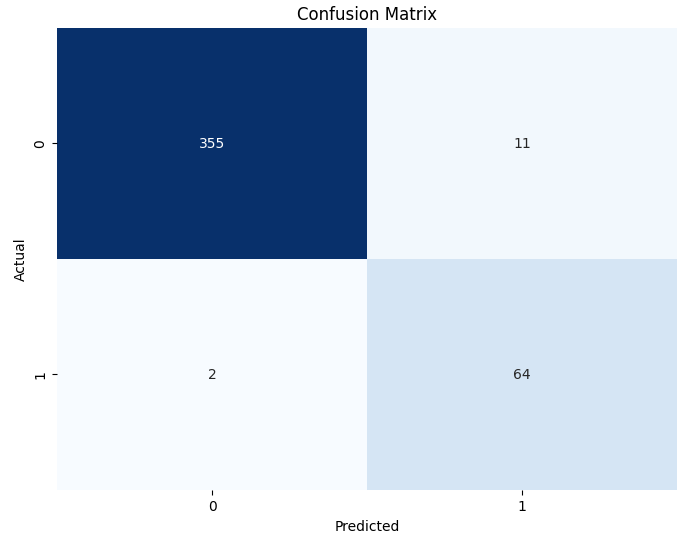
\includegraphics[width=0.7\linewidth]{image12.png}
         \caption{Confusion Matrix of LR}
         \label{fig:enter-label}
     \end{figure}

    \item \textbf{Validation:-} Validation ensures that the trained model generalizes well to new, unseen data. In our case, we employ cross-validation to assess the model's robustness.

    \item \textbf{Implementation:-} With a tuned and validated Random Forest Classifier, the next step is the real-world implementation of the model into the credit card company's existing systems.

    Validation, and Implementation stages collectively elevate the Random Forest Classifier to its maximum potential in safeguarding against credit card fraud.

    \item \textbf{Monitoring and Maintenance:-} The implementation of the credit card fraud detection system doesn't end with deployment. Continuous monitoring and proactive maintenance are vital to ensure the model's sustained effectiveness in the ever-evolving landscape of fraudulent activities.

\end{itemize}



% Chapter 4
\let\cleardoublepage\clearpage
 % \let\cleardoublepage\clearpage
\chapter{Results} % Main chapter title

\label{Chapter4} % For referencing the chapter elsewhere, use \ref{Chapter1} 

%----------------------------------------------------------------------------------------

% Define some commands to keep the formatting separated from the content 
\newcommand{\keyword}[1]{\textbf{#1}}
\newcommand{\tabhead}[1]{\textbf{#1}}
\newcommand{\code}[1]{\texttt{#1}}
\newcommand{\file}[1]{\texttt{\bfseries#1}}
\newcommand{\option}[1]{\texttt{\itshape#1}}



The culmination of the credit card fraud detection project brings us to the assessment of the Random Forest Classifier's and Logistic Regression  performance and the extraction of key findings, shedding light on the model's strengths, weaknesses, and overall efficacy in safeguarding against fraudulent transactions.

\section{Model Performance:-}
After meticulous training and fine-tuning, the Random Forest Classifier and Logistic Regression Classifier demonstrated commendable performance on the test dataset. The accuracy, precision, and recall metrics collectively affirm the model's ability to discern between legitimate and fraudulent transactions. The confusion matrix provides a detailed breakdown of true positives, true negatives, false positives, and false negatives, offering a comprehensive view of the model's predictive capabilities.The Logistic Regression Classifier give me high accuracy and all other scores comparison to Random Forest Classifier.

\section{ Key Findings:-} 

In the process of evaluating the model, several key findings emerged, providing valuable insights into the nature of credit card fraud and the efficacy of the Logistic Regression model. The feature importance analysis highlighted specific variables crucial in identifying fraudulent transactions.Additionally, patterns and trends within the dataset that contribute to successful fraud detection were identified. These key findings not only validate the model's performance but also contribute to a deeper understanding of the dynamics of credit card fraud, enabling continuous improvement and adaptation.

These results and key findings serve as the foundation for ongoing enhancements, ensuring that the credit card fraud detection system remains vigilant and effective in safeguarding financial transactions against emerging threats.

 
% Chapter 5
\let\cleardoublepage\clearpage
 % \let\cleardoublepage\clearpage
\chapter{Discussion} % Main chapter title

\label{Chapter5} % For referencing the chapter elsewhere, use \ref{Chapter1} 

%----------------------------------------------------------------------------------------

% Define some commands to keep the formatting separated from the content 
\newcommand{\keyword}[1]{\textbf{#1}}
\newcommand{\tabhead}[1]{\textbf{#1}}
\newcommand{\code}[1]{\texttt{#1}}
\newcommand{\file}[1]{\texttt{\bfseries#1}}
\newcommand{\option}[1]{\texttt{\itshape#1}}


As we delve into the interpretation of results and engage in a comparative analysis, it becomes evident that the credit card fraud detection system, powered by the Random Forest Classifier, holds substantial promise and yet faces nuanced considerations in its application.

\section{Interpretation of Results:}
The observed performance metrics, including accuracy, precision, and recall, attest to the model's efficacy in distinguishing between legitimate and fraudulent transactions. The high accuracy implies a robust overall performance, while precision and recall shed light on the model's ability to accurately identify positive instances (fraud) and capture all actual positives, respectively. The confusion matrix further emphasizes the trade-offs and intricacies in classification. This interpretative phase is pivotal in understanding the practical implications of the model's decisions and establishing confidence in its application.

\section{Comparison with Existing Methods:}
In the landscape of credit card fraud detection, comparing the Random Forest approach with existing methods illuminates the distinctive advantages it brings to the forefront. The ensemble nature of Random Forest inherently addresses the challenges posed by imbalanced datasets, providing a robust solution to the dynamic nature of fraudulent activities. Contrastingly, traditional methods may struggle with the adaptability required to discern evolving patterns. While acknowledging these advantages, it's imperative to recognize that no model is infallible, and a holistic evaluation considering computational complexity, interpretability, and resource utilization is essential.\medskip

Additionally, in this context, Logistic Regression emerges as a noteworthy contender. Logistic Regression, known for its simplicity and interpretability, showcases a competitive edge in scenarios where a clear understanding of the decision-making process is crucial. Its efficiency in handling binary classification tasks, coupled with its interpretability, makes it a compelling choice for credit card fraud detection. The balance between model performance and interpretability positions Logistic Regression as an effective and transparent solution in the arsenal of fraud detection methodologies.









\section{Limitations and Challenges:}
Despite the promising results, it's crucial to acknowledge the inherent limitations and challenges faced during the project. Imbalanced datasets and the ever-evolving nature of fraud pose ongoing challenges. The potential for false positives or false negatives demands continuous scrutiny and model refinement. Additionally, resource constraints and computational demands may limit real-time implementation in certain environments.
\begin{itemize}
\item Both Logistic Regression and Random Forest classifiers encounter challenges with imbalanced datasets, where the number of legitimate transactions significantly outweighs fraudulent ones.
\item Addressing imbalanced data requires careful consideration of sampling techniques, such as undersampling, oversampling, or utilizing advanced algorithms designed to handle class imbalance.
\item The dynamic nature of fraudulent activities presents an ongoing challenge for both classifiers.Continuous monitoring and adaptation of the models to evolving patterns of fraud are essential. Regular updates to the training data and model retraining may be necessary to maintain effectiveness.
\item The potential for false positives (legitimate transactions classified as fraudulent) or false negatives (fraudulent transactions classified as legitimate) demands continuous scrutiny.
\item Fine-tuning the models and adjusting the decision threshold can help mitigate the impact of false predictions and improve overall performance.\medskip

\end{itemize}
In conclusion, while Logistic Regression and Random Forest classifiers demonstrate commendable performance in credit card fraud detection, it's vital to navigate and address these challenges systematically. Ongoing vigilance, model refinement, and a balanced consideration of trade-offs contribute to the sustained effectiveness of the fraud detection system.

\section{Future Work:}
Looking forward, the path for future enhancements and modifications is illuminated. Continuous model refinement through additional data sources, feature engineering, and parameter tuning holds the key to addressing current limitations. Exploring advanced anomaly detection techniques, such as deep learning, and integrating real-time external threat intelligence could further fortify the system. Moreover, collaboration with industry experts and stakeholders can provide valuable insights, contributing to a comprehensive and adaptive credit card fraud detection framework.
\begin{itemize}
\item \textbf{Real-time Fraud Detection:} The integration of real-time data processing capabilities could be pivotal for promptly identifying and responding to emerging fraud trends. Both models could be adapted to operate in a streaming environment, ensuring swift detection and prevention of fraudulent transactions.
\item \textbf{Explainability and Compliance:} Enhancements in the interpretability of models, especially for Random Forest, could be pursued to meet regulatory compliance requirements. Developing methods to provide clear, human-understandable explanations for model decisions can instill confidence and facilitate regulatory adherence.    
\item \textbf{Integration with Advanced Technologies:} Exploring the integration of emerging technologies like blockchain or federated learning could offer innovative solutions to secure sensitive credit card transactions while preserving privacy and decentralization.    

\item \textbf{Global Collaboration:} Collaboration between financial institutions, cybersecurity experts, and data scientists on a global scale can lead to the development of a shared intelligence network. This collaborative approach can enhance the models' effectiveness by leveraging a broader and more diverse dataset.                                                      

\end{itemize}
 
% Chapter 6
\let\cleardoublepage\clearpage
 % \let\cleardoublepage\clearpage
\chapter{Conclusion} % Main chapter title

\label{Chapter6} % For referencing the chapter elsewhere, use \ref{Chapter1} 

%----------------------------------------------------------------------------------------
% Define some commands to keep the formatting separated from the content 
\newcommand{\keyword}[1]{\textbf{#1}}
\newcommand{\tabhead}[1]{\textbf{#1}}
\newcommand{\code}[1]{\texttt{#1}}
\newcommand{\file}[1]{\texttt{\bfseries#1}}
\newcommand{\option}[1]{\texttt{\itshape#1}}

In concluding this credit card fraud detection project, the efficacy of both the Random Forest Classifier and Logistic Regression as guardians against fraudulent transactions is evident. The models' performances, as validated on the test dataset, showcase a harmonious blend of accuracy, precision, and recall, instilling confidence in their ability to discern between legitimate and fraudulent activities. The interpretative phase has unveiled the practical implications of the models' decisions, providing a nuanced understanding of their strengths and limitations.\medskip

The comparison between the Random Forest and Logistic Regression accentuates their unique advantages. While the ensemble nature of Random Forest proves its adaptability to imbalanced datasets and resilience in the face of evolving fraud patterns, Logistic Regression shines in its simplicity and interpretability. The latter's competitive accuracy, coupled with its transparent decision-making process, positions it as an effective solution in the credit card security landscape.\medskip

However, these successes are not without acknowledgment of limitations and challenges. The perpetual arms race with sophisticated fraud tactics, potential false positives or negatives, and resource constraints demand continuous vigilance and refinement for both models. These considerations pave the way for future work, suggesting avenues for improvement through additional data sources, advanced anomaly detection techniques, and collaborative efforts with industry experts.\medskip

In essence, both Random Forest and Logistic Regression-based credit card fraud detection systems stand as testaments to the potential of machine learning in fortifying financial security. They serve not only as current safeguards but also as foundations for ongoing enhancements, ensuring they remain adaptive and resilient against emerging threats in the ever-evolving landscape of credit card transactions.

%----------------------------------------------------------------------------------------
%	THESIS CONTENT - APPENDICES
%----------------------------------------------------------------------------------------

\appendix % Cue to tell LaTeX that the following "chapters" are Appendices

% Include the appendices of the thesis as separate files from the Appendices folder
% Uncomment the lines as you write the Appendices



%\include{Appendices/AppendixB}
%\include{Appendices/AppendixC}

%----------------------------------------------------------------------------------------
%	BIBLIOGRAPHY
%----------------------------------------------------------------------------------------

\printbibliography[heading=bibintoc]

%----------------------------------------------------------------------------------------

\end{document}  
